\documentclass[11pt,fleqn]{article}
\usepackage[letterpaper]{geometry}
\usepackage{graphicx}    % needed for including graphics e.g. EPS, PS
\usepackage{amsmath}
\usepackage{xfrac}
\usepackage[version=4]{mhchem}
\usepackage{listings}
\usepackage{hyperref}
\usepackage{wrapfig}
\usepackage{empheq}



% To use UTF-8 characters
\usepackage[utf8x]{inputenc}
% \DeclareUnicodeCharacter{207A}{$^+$}
% \DeclareUnicodeCharacter{207B}{$^-$}

\usepackage{tikz}


\topmargin -1.5cm        % read Lamport p.163
\oddsidemargin -0.04cm   % read Lamport p.163
\evensidemargin -0.04cm  % same as oddsidemargin but for left-hand pages
\textwidth 16.59cm
\textheight 21.94cm 
%\pagestyle{empty}       % Uncomment if don't want page numbers
\parskip 7.2pt           % sets spacing between paragraphs
%\renewcommand{\baselinestretch}{1.5} 	% Uncomment for 1.5 spacing between lines
\parindent 0pt		  % sets leading space for paragraphs


\newcounter{qNum}
\newcommand{\qn}{\refstepcounter{qNum} \theqNum}
\newcounter{qNumH}
\newcommand{\qnH}{\refstepcounter{qNumH}  \textit{Honors} \theqNumH}
\newcommand{\eqn}{\text{\qn) \ }}
\def \dt {\ensuremath{\,\mathrm{d}t}}

\newcommand{\aspace}{ \hspace{1em}\\ \vspace{8em}}

\newcommand{\dx}{\; dx}

\newcommand{\D}[1]{\; d{#1}}

\newcommand{\graphGrid}{
	
\begin{tikzpicture}
	\draw[step=.5cm,gray,help lines] (-5,-5) grid (5,5);
	\draw[step=2.5cm,black,very thin] (-5,-5) grid (5,5);
	\end{tikzpicture}
}

\newcommand{\graphGridAxes}{
	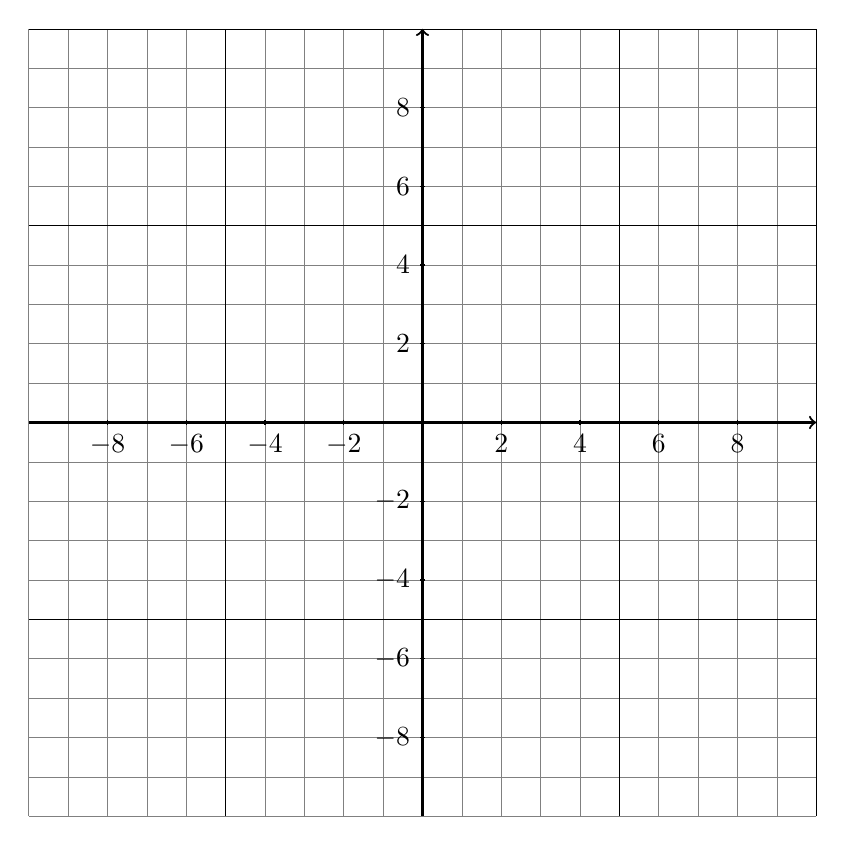
\begin{tikzpicture}
	\draw[step=.5cm,gray,help lines] (-5,-5) grid (5,5);
	\draw[step=2.5cm,black,very thin] (-5,-5) grid (5,5);
	\draw[thick,->] (-5,0) -- (5,0) ;
	\draw[thick,->] (0,-5) -- (0,5) ; 
	\foreach \x in {-8, -6, -4, -2,  2,4, 6, 8}
	\draw (\x*0.5 cm,1pt) -- (\x*0.5 cm,-1pt) node[anchor=north] {$\x$};
	\foreach \y in {-8, -6, -4, -2,  2,4, 6, 8}
	\draw (1pt,\y*0.5 cm) -- (-1pt,\y*0.5 cm) node[anchor=east] {$\y$};
	\end{tikzpicture}
}

\newcommand{\graphGridAxesS}[1]{
	\begin{tikzpicture}
		\draw[step=.5cm,gray,help lines] (-0.5*#1,-0.5*#1) grid (0.5*#1, 0.5*#1);
		\draw[step=2.5cm,black,very thin] (-0.5*#1,-0.5*#1) grid (0.5*#1, 0.5*#1);
		\draw[thick,->] (-#1/2,0) -- (#1/2,0) ;
		\draw[thick,->] (0,-#1/2) -- (0,#1/2) ; 
		\foreach \x in {-8, -6, -4, -2,  2,4, 6, 8}
		\draw (\x*0.5 cm,1pt) -- (\x*0.5 cm,-1pt) node[anchor=north] {$\x$};
		\foreach \y in {-8, -6, -4, -2,  2,4, 6, 8}
		\draw (1pt,\y*0.5 cm) -- (-1pt,\y*0.5 cm) node[anchor=east] {$\y$};
	\end{tikzpicture}
}



%headers
\usepackage{datetime}
\usepackage{fancyhdr}
\pagestyle{fancy}
\lhead{ Name: }
\rhead{\footnotesize Finite Difference Method: Cylindrical Tube (\monthname, \the\year)}
\title{Introduction to the Finite Difference Method: \\ Filling and Draining a Cylindrical Tube}
\author{Lensyl Urbano}



 \begin{document}         
 % Start your text
 
\maketitle



Consider filling a cylinder with water. The water flows in at a constant rate of 5 cm$^3$/s. The inflow rate can be written as the change in volume over the change in time:

\begin{equation}
	\frac{dV}{dt} = 5 \; cm^3/s
\end{equation}

\begin{wrapfigure}{r}{0.5\textwidth}
	\begin{center}
		
		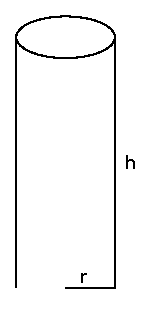
\includegraphics{cylinder-rh-i.pdf}
		\caption{Cylindrical tube for filling and draining. $r$ is the radius and $h$ is the height.}
		
	\end{center}
\end{wrapfigure}

\section{Filling the Tube}

\subsection{Conceptual Physics Approach}

	      
So, at this inflow rate, after 10 seconds there will be 50 cm$^3$ added to the cylinder.

	\begin{align*}
		 V &= 5 \; cm^3/s \cdot 10 \; s \\
				&= 50 \; cm^3
	\end{align*}

In terms of the equation, the change in volume is equal to the inflow rate ($\frac{dV}{dt}$) times the time period ($ t$).

  \begin{equation}
  	\label{Vrate}
  	 V = \frac{dV}{d t} \cdot t \\
  \end{equation}

How high will the water have risen in the cylinder in those 10 seconds when 50 cm$^3$ of water was added? Well, we know that the volume of a cylinder is given by the equation:

	\begin{equation}
		V = \pi r^2 h
	\end{equation}

So, if we know the volume and the radius of the cylinder ($r$) we can solve this equation for the height:

	\begin{align}
		V &= \pi r^2 h \\
		\frac{V}{\pi r^2} &= \frac{\pi r^2 h}{\pi r^2} \\
	    \frac{V}{\pi r^2} &= h  \\
		h &= \frac{V}{\pi r^2} 
	\end{align}


Now we can substitute the volume from Equation \ref{Vrate} to get:

	\begin{equation}
		h = \frac{\frac{dV}{d t} \cdot t}{\pi r^2}
	\end{equation}

Finally, lets rewrite this in terms of the change from moment to moment: the change in height ($\Delta h$) instead of height ($h$) over a given change in time ($\Delta t$) instead of the absolute time ($t$):

	\begin{empheq}[box=\fbox]{equation}
		\label{dh_eqn}
		\Delta h = \frac{\frac{dV}{d t} \cdot \Delta t}{\pi r^2}
	\end{empheq}

Having calculated the change in the height of the water in the cylinder in a given time step ($\Delta t$), for each timestep we calculate the new height of water ($h_{new}$) as the old height plus the change:

	\begin{empheq}[box=\fbox]{equation}
		\label{hnew_eqn}
		h_{new} = h_{old} + \Delta h
	\end{empheq}


\subsection{Using Calculus to Find the Discrete Equations} \label{CodeCalc}

	Same problem--filling a cylinder--but using calculus to end up with the same equations in the end.
	
	Start with the equation for the volume of a cylinder:
	
		\begin{equation}
			V = \pi r^2 h
		\end{equation}
	
	There are two variables that change with time as the cylinder fills, the volume ($V$) and the height ($h$) since the radius ($r$) does not change. So, if we differentiate this equation with respect to time (implicit differentiation), we get:
		\begin{equation}
			\frac{dV}{dt} = \pi r^2 \frac{dh}{dt} 
		\end{equation}
	
	Solving for $\frac{dh}{dt}$:
		\begin{equation}
			\frac{dh}{dt} = \frac{\frac{dh}{dt} }{\pi r^2 }
		\end{equation}
	
	%And solving for $dh$ gives:
	%	\begin{equation}
	%		dh = \frac{\frac{dh}{dt} \cdot dt }{\pi r^2 }
	%	\end{equation}
	
	However, what if we switched from the instantaneous change in height with time ($\frac{dh}{dt}$) to the discrete change ($\frac{\Delta h}{\Delta t}$) we get:
		\begin{equation}
			\frac{\Delta h}{\Delta t} = \frac{\frac{dh}{dt} }{\pi r^2 }
		\end{equation}
		
	which we can solve for the change in height ($\Delta h$):
		\begin{equation}
			\Delta h = \frac{\frac{dh}{dt} \cdot \Delta t }{\pi r^2 }
		\end{equation}
	
	As we know, the discrete change can be written as a difference between two values: e.g. $\Delta x = x_2 - x_1$. So, we rewrite $\Delta h$ as:
		\begin{equation}
			\Delta h = h_{new} - h_{old}
		\end{equation}
	
	Which we can solve for the new height:
		\begin{equation}
			h_{new} = h_{old} + \Delta h 
		\end{equation}
	
	We thus end up with the same equation as before.

\newpage
\subsection{Code}

	The following example code that solves this water-filling problem uses the \href{https://github.com/lurbano/ezGraph}{ezGraph class} \\ (https://github.com/lurbano/ezGraph) which requires matplotlib and numpy. However, the code in the following section avoids the use of most imported modules, but does not graph.
	
	\subsubsection{Code with Graphical Output}
	\textit{water-filling-fd.py}
\begin{lstlisting}[frame=single]
import numpy as np 
import time 
from ezGraph import *

# Finite Difference Model

# PARAMETERS
dt = 1.
nsteps = 20

r = 2.25    # radius (cm)
Q = 5       # Volume inflow rate: (cubic cm / s)
h = 0       # Initial height (cm)

# GRAPH
graph = ezGraph(xmax=30, ymin=0, ymax=10, 
          xLabel="Time (s)", yLabel="Height (cm)")
graph.add(0, h)             # add initial values


# TIME LOOP
for t in range(1, nsteps):
modelTime = t * dt

dh = Q * dt / (np.pi * r**2)    # find the change in height
h = h + dh                      # update height

print(modelTime, h)
graph.add(modelTime, h)
graph.wait(0.1)

# DRAW GRAPH
graph.keepOpen()
	
	
\end{lstlisting}
	
	\begin{figure} 
		\caption{Model output: Graph of height of water in the column over time when filling the cylinder.}
		\centering
		\label{fillingModel}
		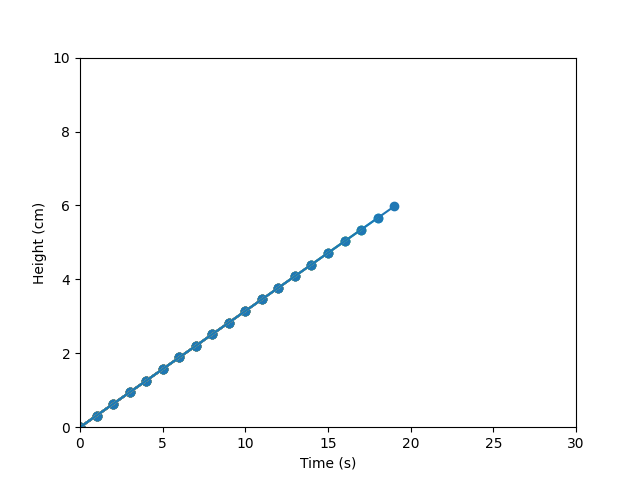
\includegraphics[width=0.75\textwidth]{water-filling-fd.png}
	\end{figure}
	
	\subsection{Code without Graphical Output}
	A stripped down version of the code with no graph and no external modules except "math".
	
	\textit{water-filling-fd-noGraph.py}
\begin{lstlisting}[frame=single]
import math
# Finite Difference Model

# PARAMETERS
dt = 1.
nsteps = 20

r = 2.25    # radius (cm)
Q = 5       # Volume inflow rate: (cubic cm / s)
h = 0       # Initial height (cm)

print(0, h)     # print initial values

# TIME LOOP
for t in range(1, nsteps):
modelTime = t * dt

dh = Q * dt / (math.pi * r**2)  # find the change in height
h = h + dh                      # update height

print(modelTime, h)
	
\end{lstlisting}
	
	Which should produce a table of time and height output:
	
	\begin{lstlisting}
		0 0
		1.0 0.31438013450250935
		2.0 0.6287602690050187
		3.0 0.943140403507528
		4.0 1.2575205380100374
		5.0 1.5719006725125468
		6.0 1.8862808070150563
		7.0 2.2006609415175657
		8.0 2.515041076020075
		9.0 2.8294212105225847
		10.0 3.143801345025094
		11.0 3.4581814795276036
		12.0 3.772561614030113
		13.0 4.086941748532622
		14.0 4.4013218830351315
		15.0 4.715702017537641
		16.0 5.03008215204015
		17.0 5.34446228654266
		18.0 5.658842421045169
		19.0 5.973222555547679
	\end{lstlisting}



\section{Analytical Solutions using Calculus}

	\subsection{Filling}

	As we saw in the section on using calculus (Section \ref{CodeCalc}), we can start with the equation for the volume of a cylinder:
	\begin{equation}
		V = \pi r^2 h
	\end{equation}
	
	And differentiate with respect to time to get:
	\begin{equation}
		\frac{dV}{dt} = \pi r^2 \frac{dh}{dt} 
	\end{equation}

	Assuming a constant inflow rate ($\frac{dV}{dt} = Q$):
	\begin{equation}
		Q = \pi r^2 \frac{dh}{dt} 
	\end{equation}

	And solve for $\frac{dh}{dt}$:
	\begin{equation}
		\frac{dh}{dt} = \frac{Q}{\pi r^2 }
	\end{equation}

	This we can separate:
	\begin{equation}
		dh = \frac{Q}{\pi r^2 } dt
	\end{equation}
	
	and integrate:
	\begin{equation}
		\int{dh} = \int{\frac{Q}{\pi r^2 } dt}
	\end{equation}

	to get:
	\begin{equation}
		h = \frac{Q}{\pi r^2 } t + c
	\end{equation}

	When $t=0$, $c$ can be shown to be the initial height ($c = h_i$) so:
	\begin{equation}
		h = \frac{Q}{\pi r^2 } t + h_i
	\end{equation}

	And since $\frac{Q}{\pi r^2}$ is constant, we can see that this term is the slope in a linear equation of the form.
	\begin{equation}
		y = mx + b
	\end{equation}

	So the linear pattern produced by the filling model is correct (Figure \ref{fillingModel}).


\section{Draining}

	\subsection{Draining: Analytical Solution using Calculus}
	Experiments (which you may have done) show that if you're draining a cylinder by gravity the outflow rate of water is linearly proportional to the height of water in the tube. 
	\begin{equation}
		\frac{dV}{dt} \propto h
	\end{equation}

	Converting the proportionality statement to an equation requires us to introduce a constant ($k$):
	\begin{equation}
		\label{DrainingDiffEqn}
		\frac{dV}{dt} = k h
	\end{equation}

	So in draining, the outflow rate ($\frac{dV}{dt}$) is not constant, it slows down as the height of water in the tube decreases. 
	
	Now, lets substitute the equation for the volume of a cylinder:
	
	\begin{equation}
		V = \pi r^2 h
	\end{equation}
	
	into the draining equation (Eq. \ref{DrainingDiffEqn}) to get:
	
	\begin{equation}
		\frac{d[\pi r^2 h]}{dt} = k h
	\end{equation}

	we can extract $\pi$ and $r^2$ from the differential because they are constant:
	\begin{equation}
		\pi r^2 \frac{dh}{dt} = k h
	\end{equation}

	separating the variables gives:
	\begin{equation}
		\pi r^2 \frac{dh}{h} = k \cdot dt
	\end{equation}
	and rearranging:
	\begin{equation}
		\frac{dh}{h} = \frac{k \cdot dt}{\pi r^2 }
	\end{equation}
	\begin{equation}
		\frac{dh}{h} = \frac{k}{\pi r^2 } dt
	\end{equation}

	To simplify a little, lets consolidate the constants on the left hand side into one therm $K$:
	\begin{equation}
		K = \frac{k}{\pi r^2 }
	\end{equation}
	so:
	\begin{equation}
		\frac{dh}{h} = K \cdot dt 
	\end{equation}
	
	which we can integrate (remember $K$ is a constant):
	\begin{align}
		\int \frac{dh}{h} &= K \int dt \\
		\ln{h} &= K \cdot t + c
	\end{align}
	
	we can solve for $h$ by raising both sides by $e$ to cancel the $\ln$:
	\begin{equation}
		e^{\ln{h}} = e^{K t + c}
	\end{equation}

	\begin{equation}
		h = e^{K t + c}
	\end{equation}

	Because of math, we can pull the constant out to get:
	\begin{equation}
		h = Ce^{K t}
	\end{equation}

	Where the constant is the initial value of the height ($h_0$):
	\begin{equation}
		\label{analyticalDraining}
		h = h_0 \cdot e^{K t}
	\end{equation}

	This is an exponential function. If $K$ is less than 1 ($K<1$) then this is a decay curve.
	
	
	\subsection{Numerical Solution}
	
	For draining, the outflow rate (change in volume over time, $\frac{dV}{dt}$) is not constant. The outflow rate is proportional to the height of water in the tube, since the higher the water level the greater pressure at the bottom of the tube and the faster the outflow rate.
	\begin{equation}
		\frac{dV}{dt} \propto h
	\end{equation}
	
	Converting the proportionality statement to an equation requires us to introduce a constant ($k$):
	\begin{equation}
		\label{DrainingDiffEqn}
		\frac{dV}{dt} = k \cdot h
	\end{equation}

	So, let's substitute this relationship into the height change equation (Eq. \ref{dh_eqn}):
	\begin{empheq}[]{equation*}
		\Delta h = \frac{\frac{dV}{d t} \cdot \Delta t}{\pi r^2}
	\end{empheq}
	
	to get:
	\begin{empheq}[box=\fbox]{equation}
		\Delta h = \frac{k \cdot h \cdot \Delta t}{\pi r^2}
	\end{empheq}

	so, in our code we just need to change this line and set up a few different constants.
	
	
	
	\subsection{Code: Draining}
	
	This program is based off the filling code. We're using an initial height of 50 cm ($h_i = 50$), and set the constant $K=1$.
	
\textit{water-draining-fd.py}
\begin{lstlisting}[frame=single]
import numpy as np 
import time 
from ezGraph import *

# Finite Difference Model

# PARAMETERS
dt = 1
nsteps = 100

r = 2.25    # radius (cm)
Q = 0       # Volume inflow rate (dV/dt): (cubic cm / s)
h = 50       # Initial height (cm)
k = 1.0     # outflow rate constant

# GRAPH
graph = ezGraph(xmax=100, 
xLabel="Time (s)", yLabel="Height (cm)")
graph.add(0, h)             # add initial values


# TIME LOOP
for t in range(1, nsteps):
modelTime = t * dt

# Filling
dh = Q * dt / (np.pi * r**2)    # find the change in height
h = h + dh                      # update height

# Draining
dVdt = -k * h
dh = dVdt * dt / (np.pi * r**2)
h = h + dh

print(modelTime, h)
graph.add(modelTime, h)
graph.wait(0.1)

# DRAW GRAPH
graph.keepOpen()


\end{lstlisting}
	
	
	\begin{figure} 
		\caption{Model output: Graph of height of water in the column over time when draining the cylinder.}
		\centering
		\label{drainingModel}
		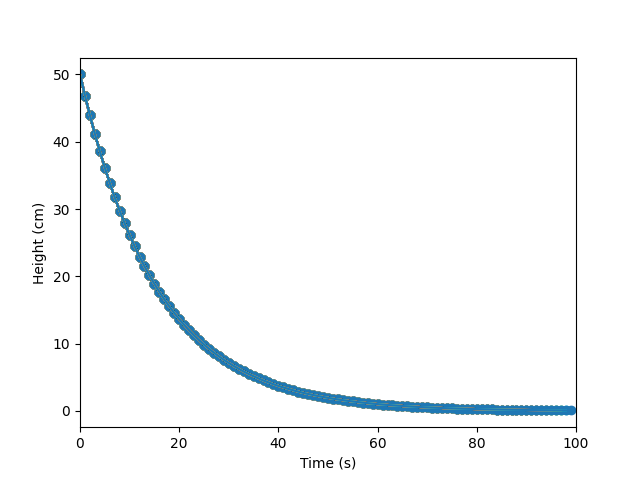
\includegraphics[width=0.75\textwidth]{water-draining-fd.png}
	\end{figure}

The output from the model (Fig. \ref{drainingModel}) looks like an exponential decay curve, which is what we find from the analytical solution (Eqn. \ref{analyticalDraining}).

 % Stop your text
 \end{document}
